\documentclass[]{article}
\usepackage{lmodern}
\usepackage{amssymb,amsmath}
\usepackage{ifxetex,ifluatex}
\usepackage{fixltx2e} % provides \textsubscript
\ifnum 0\ifxetex 1\fi\ifluatex 1\fi=0 % if pdftex
  \usepackage[T1]{fontenc}
  \usepackage[utf8]{inputenc}
\else % if luatex or xelatex
  \ifxetex
    \usepackage{mathspec}
  \else
    \usepackage{fontspec}
  \fi
  \defaultfontfeatures{Ligatures=TeX,Scale=MatchLowercase}
\fi
% use upquote if available, for straight quotes in verbatim environments
\IfFileExists{upquote.sty}{\usepackage{upquote}}{}
% use microtype if available
\IfFileExists{microtype.sty}{%
\usepackage{microtype}
\UseMicrotypeSet[protrusion]{basicmath} % disable protrusion for tt fonts
}{}
\usepackage[margin=1in]{geometry}
\usepackage{hyperref}
\hypersetup{unicode=true,
            pdftitle={CM 2.1-2 - Simple linear regression},
            pdfborder={0 0 0},
            breaklinks=true}
\urlstyle{same}  % don't use monospace font for urls
\usepackage{color}
\usepackage{fancyvrb}
\newcommand{\VerbBar}{|}
\newcommand{\VERB}{\Verb[commandchars=\\\{\}]}
\DefineVerbatimEnvironment{Highlighting}{Verbatim}{commandchars=\\\{\}}
% Add ',fontsize=\small' for more characters per line
\usepackage{framed}
\definecolor{shadecolor}{RGB}{248,248,248}
\newenvironment{Shaded}{\begin{snugshade}}{\end{snugshade}}
\newcommand{\AlertTok}[1]{\textcolor[rgb]{0.94,0.16,0.16}{#1}}
\newcommand{\AnnotationTok}[1]{\textcolor[rgb]{0.56,0.35,0.01}{\textbf{\textit{#1}}}}
\newcommand{\AttributeTok}[1]{\textcolor[rgb]{0.77,0.63,0.00}{#1}}
\newcommand{\BaseNTok}[1]{\textcolor[rgb]{0.00,0.00,0.81}{#1}}
\newcommand{\BuiltInTok}[1]{#1}
\newcommand{\CharTok}[1]{\textcolor[rgb]{0.31,0.60,0.02}{#1}}
\newcommand{\CommentTok}[1]{\textcolor[rgb]{0.56,0.35,0.01}{\textit{#1}}}
\newcommand{\CommentVarTok}[1]{\textcolor[rgb]{0.56,0.35,0.01}{\textbf{\textit{#1}}}}
\newcommand{\ConstantTok}[1]{\textcolor[rgb]{0.00,0.00,0.00}{#1}}
\newcommand{\ControlFlowTok}[1]{\textcolor[rgb]{0.13,0.29,0.53}{\textbf{#1}}}
\newcommand{\DataTypeTok}[1]{\textcolor[rgb]{0.13,0.29,0.53}{#1}}
\newcommand{\DecValTok}[1]{\textcolor[rgb]{0.00,0.00,0.81}{#1}}
\newcommand{\DocumentationTok}[1]{\textcolor[rgb]{0.56,0.35,0.01}{\textbf{\textit{#1}}}}
\newcommand{\ErrorTok}[1]{\textcolor[rgb]{0.64,0.00,0.00}{\textbf{#1}}}
\newcommand{\ExtensionTok}[1]{#1}
\newcommand{\FloatTok}[1]{\textcolor[rgb]{0.00,0.00,0.81}{#1}}
\newcommand{\FunctionTok}[1]{\textcolor[rgb]{0.00,0.00,0.00}{#1}}
\newcommand{\ImportTok}[1]{#1}
\newcommand{\InformationTok}[1]{\textcolor[rgb]{0.56,0.35,0.01}{\textbf{\textit{#1}}}}
\newcommand{\KeywordTok}[1]{\textcolor[rgb]{0.13,0.29,0.53}{\textbf{#1}}}
\newcommand{\NormalTok}[1]{#1}
\newcommand{\OperatorTok}[1]{\textcolor[rgb]{0.81,0.36,0.00}{\textbf{#1}}}
\newcommand{\OtherTok}[1]{\textcolor[rgb]{0.56,0.35,0.01}{#1}}
\newcommand{\PreprocessorTok}[1]{\textcolor[rgb]{0.56,0.35,0.01}{\textit{#1}}}
\newcommand{\RegionMarkerTok}[1]{#1}
\newcommand{\SpecialCharTok}[1]{\textcolor[rgb]{0.00,0.00,0.00}{#1}}
\newcommand{\SpecialStringTok}[1]{\textcolor[rgb]{0.31,0.60,0.02}{#1}}
\newcommand{\StringTok}[1]{\textcolor[rgb]{0.31,0.60,0.02}{#1}}
\newcommand{\VariableTok}[1]{\textcolor[rgb]{0.00,0.00,0.00}{#1}}
\newcommand{\VerbatimStringTok}[1]{\textcolor[rgb]{0.31,0.60,0.02}{#1}}
\newcommand{\WarningTok}[1]{\textcolor[rgb]{0.56,0.35,0.01}{\textbf{\textit{#1}}}}
\usepackage{graphicx,grffile}
\makeatletter
\def\maxwidth{\ifdim\Gin@nat@width>\linewidth\linewidth\else\Gin@nat@width\fi}
\def\maxheight{\ifdim\Gin@nat@height>\textheight\textheight\else\Gin@nat@height\fi}
\makeatother
% Scale images if necessary, so that they will not overflow the page
% margins by default, and it is still possible to overwrite the defaults
% using explicit options in \includegraphics[width, height, ...]{}
\setkeys{Gin}{width=\maxwidth,height=\maxheight,keepaspectratio}
\IfFileExists{parskip.sty}{%
\usepackage{parskip}
}{% else
\setlength{\parindent}{0pt}
\setlength{\parskip}{6pt plus 2pt minus 1pt}
}
\setlength{\emergencystretch}{3em}  % prevent overfull lines
\providecommand{\tightlist}{%
  \setlength{\itemsep}{0pt}\setlength{\parskip}{0pt}}
\setcounter{secnumdepth}{0}
% Redefines (sub)paragraphs to behave more like sections
\ifx\paragraph\undefined\else
\let\oldparagraph\paragraph
\renewcommand{\paragraph}[1]{\oldparagraph{#1}\mbox{}}
\fi
\ifx\subparagraph\undefined\else
\let\oldsubparagraph\subparagraph
\renewcommand{\subparagraph}[1]{\oldsubparagraph{#1}\mbox{}}
\fi

%%% Use protect on footnotes to avoid problems with footnotes in titles
\let\rmarkdownfootnote\footnote%
\def\footnote{\protect\rmarkdownfootnote}

%%% Change title format to be more compact
\usepackage{titling}

% Create subtitle command for use in maketitle
\providecommand{\subtitle}[1]{
  \posttitle{
    \begin{center}\large#1\end{center}
    }
}

\setlength{\droptitle}{-2em}

  \title{CM 2.1-2 - Simple linear regression}
    \pretitle{\vspace{\droptitle}\centering\huge}
  \posttitle{\par}
  \subtitle{Math 530/630}
  \author{}
    \preauthor{}\postauthor{}
    \date{}
    \predate{}\postdate{}
  

\begin{document}
\maketitle

{
\setcounter{tocdepth}{2}
\tableofcontents
}
\hypertarget{overview}{%
\section{Overview}\label{overview}}

\begin{itemize}
\tightlist
\item
  A complete knitted \texttt{html} file is due on Sakai by the beginning
  of the next class.
\item
  This lab is based on
  \href{https://moderndive.com/5-regression.html}{Chapter 5: Basic
  Regression in ModernDive}. Please open it and follow closely!
\item
  You'll need to load these packages to do the lab (make sure they are
  installed first, not in your .Rmd file!):
\end{itemize}

\begin{Shaded}
\begin{Highlighting}[]
\KeywordTok{library}\NormalTok{(moderndive)}
\KeywordTok{library}\NormalTok{(tidyverse)}
\KeywordTok{library}\NormalTok{(skimr)}
\end{Highlighting}
\end{Shaded}

\hypertarget{the-data}{%
\section{The data}\label{the-data}}

Source: John Clay (1856). ``On the Relation Between Crime, Popular
Instruction, Attendance on Religious Worship, and Beer-Houses'', Journal
of the Statistical Society of London, Vol. 20 \#1, pp 22-32.

In 1856, the Reverend John Clay felt that it was high time to figure out
what societal factors were playing a role in the incidence of criminal
behavior in Britain. He stated that:

\begin{quote}
``It is a mere truism to say that the progress of popular education, and
the formation of religious habits, are fatally opposed by the
temptations to animal pleasures, which abound wherever BEER-HOUSES and
low ALE-HOUSES abound.''
\end{quote}

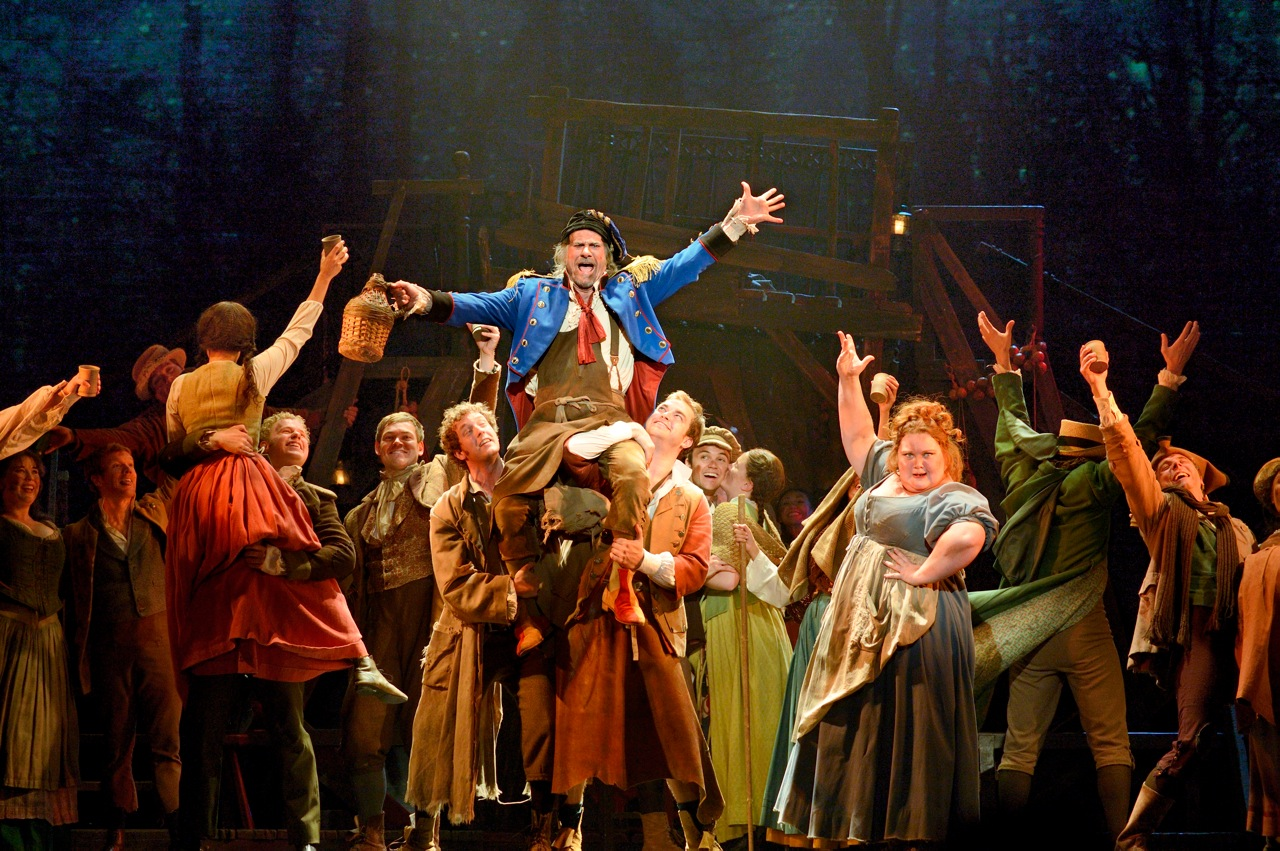
\includegraphics{../images/03.LesMiserables.US.MasteroftheHouse.jpg}

Clearly, the reverend considered public houses in Britain to be a
scourge on society, namely that they ``promote drunkenness and its
consequent evil'' (i.e., crime). Let's investigate how well we can
predict criminals (per 100k population) from the number of public houses
(ale/beer houses per 100k population) using simple linear regression.

You'll first need to download the data from the
\href{https://ohsu-math630-fall-2019.netlify.com/reference.html}{Reference
Plus (scroll down to Data Sets)} page on the course website into a
``data'' directory in your RStudio project. Assuming that, here is how
to read in the data into the crime object:

\begin{Shaded}
\begin{Highlighting}[]
\NormalTok{crimenames <-}\StringTok{ }\KeywordTok{c}\NormalTok{(}\StringTok{"county"}\NormalTok{, }\StringTok{"region_name"}\NormalTok{, }\StringTok{"region_code"}\NormalTok{,}
               \StringTok{"criminals"}\NormalTok{, }\StringTok{"public_houses"}\NormalTok{, }\StringTok{"school_attendance"}\NormalTok{,}
               \StringTok{"worship_attendance"}\NormalTok{)}

\CommentTok{# The below assumes that you've downloaded the `beerhall.dat` file to your RStudio project, into a directory named `data`.}
\NormalTok{crime <-}\StringTok{ }\KeywordTok{read_table}\NormalTok{(here}\OperatorTok{::}\KeywordTok{here}\NormalTok{(}\StringTok{"data"}\NormalTok{, }\StringTok{"beerhall.dat"}\NormalTok{),}
                    \DataTypeTok{col_names =}\NormalTok{ crimenames)}
\end{Highlighting}
\end{Shaded}

\hypertarget{basics}{%
\section{Basics}\label{basics}}

Note: you don't need to use R to answer these questions, but please
create a section header using markdown format (\texttt{\#\ Basics}) and
type your answers there.

\begin{itemize}
\tightlist
\item
  What is the dependent variable?
\item
  What is the independent variable?
\item
  Copy and paste the provided equation that starts/ends with
  \texttt{\$\$} into your narrative (not an R code chunk), and replace
  \texttt{y} and \texttt{x} in this formula with meaningful variable
  names (you may wish to reference the \texttt{crimenames} object we
  made above):
  \texttt{\$\$\textbackslash{}hat\{y\}\ =\ b\_0\ +\ b\_1\{x\}\$\$} 
\end{itemize}

\[\hat{criminals = b_0 + b_1{\textit{public_houses}}\] - The
``best-fitting'' regression line is ``best'' in that it minimizes what?
- Why is this method called ``simple linear regression'' (as opposed to
the method in
\href{http://moderndive.com/6-multiple-regression.html}{Chapter 6})?

\hypertarget{eda}{%
\section{EDA}\label{eda}}

Conduct a \href{https://moderndive.com/5-regression.html\#model1EDA}{new
exploratory data analysis}, which involves three things:

\begin{itemize}
\tightlist
\item
  Looking at the raw values.
\item
  Computing summary statistics of the variables of interest.
\item
  Creating informative visualizations.
\end{itemize}

\hypertarget{look-at-the-data}{%
\subsection{Look at the data}\label{look-at-the-data}}

Use \texttt{dplyr} to figure out how many counties are in this dataset,
and which variable names map onto the independent and dependent
variables you identified above.

\hypertarget{look-at-summary-statistics}{%
\subsection{Look at summary
statistics}\label{look-at-summary-statistics}}

Use \texttt{select} to select only the independent and dependent
variables you identified above, then pipe those variables to the
\texttt{skim} function from the \texttt{skimr} package (you should have
loaded this package at the top) to see summary statistics for each. Use
\texttt{dplyr::summarize} to calculate the correlation coefficient.

\hypertarget{visualize-the-data}{%
\subsection{Visualize the data}\label{visualize-the-data}}

Recreate the scatterplot below of ale/beer houses per 100K on the x-axis
and criminals per 100K population on the y-axis. What can you say about
the relationship between public houses and criminals based on this
exploration?

\includegraphics{cm021-2_lab-solutions_files/figure-latex/crime_scatterplot-1.pdf}

\hypertarget{simple-linear-regression-see-here}{%
\section{\texorpdfstring{Simple linear regression: (see
\href{https://moderndive.com/5-regression.html\#model1table}{here})}{Simple linear regression: (see here)}}\label{simple-linear-regression-see-here}}

\textbf{Part 1:} First ``fit'' the linear regression model to the data
using the \texttt{lm()} function, then apply the
\texttt{get\_regression\_table()} function from the \texttt{moderndive}
R package to the model object. Use the output to fill in this formula
with \texttt{y}, \texttt{x}, and the intercept and slope coefficients:
(copy and paste into your narative:
\texttt{\$\$\textbackslash{}hat\{y\}\ =\ b\_0\ +\ b\_1\{x\}\$\$})

\[\hat{y} = b_0 + b_1{x}\]

\textbf{Part 2:} Interpret the intercept coefficient and the slope
coefficient. How do the regression results match up with the results
from your exploratory data analysis above?

\hypertarget{observedfitted-values-see-here}{%
\section{\texorpdfstring{Observed/fitted values: (see
\href{http://moderndive.com/5-regression.html\#model1points}{here})}{Observed/fitted values: (see here)}}\label{observedfitted-values-see-here}}

\textbf{Part 1:} What are the observed and fitted values for the
Cornwall (\texttt{ID} = 20) and Monmouth regions (\texttt{ID} = 23)?
Which region do you think the reverend called ``the happiest example of
the infrequency of crime''?

\textbf{Part 2:} In fact, we could argue with the reverend about the
happiest example of the infrequency of crime. There are two ways you
could define this. The first way is that the county had the lowest
criminals overall. The second is that the county had the lowest
criminals \emph{given their number of public houses}. This would mean
that the region has the lowest observed criminals, compared to the
fitted value based on predicting criminals from public houses.

Filter the regression ouput using \texttt{filter} and the
\texttt{\textbar{}} operator (think: \texttt{or}) to extract the two
alternative definitions above. You'll need to match the \texttt{ID}
column as a row in the original data (you can just do this visually by
comparing the tibbles and typing your answers in your narrative- you
don't have to do a join here).

\hypertarget{residual-analysis-see-here}{%
\section{\texorpdfstring{Residual analysis: (see
\href{http://moderndive.com/5-regression.html\#model1points}{here})}{Residual analysis: (see here)}}\label{residual-analysis-see-here}}

\textbf{Part 1:} Perform a residual analysis and look for any systematic
patterns in the residuals. Ideally, there should be little to no
pattern- why? Does it seem like there is no systematic pattern to the
residuals?

\textbf{Part 2:} Recreate this density plot of the residuals. Recall
that we would like the residuals to be normally distributed with mean 0
(hint: \texttt{?geom\_vline()}). Use \texttt{dplyr} to calculate the
mean of the residuals- is it (pretty close to) 0? Do you think you have
more positive residuals than negative, or vice versa?

\includegraphics{cm021-2_lab-solutions_files/figure-latex/crime_resid_density-1.pdf}


\end{document}
